\documentclass{beamer}
\usetheme{Boadilla}
\usepackage{ifpdf}
\ifpdf
\usepackage[utf8]{inputenc}
\usepackage[T1]{fontenc}
\usepackage[all,pdf,2cell]{xy}\UseAllTwocells\SilentMatrices
\else
\usepackage[all,xdvi,2cell]{xy}\UseAllTwocells\SilentMatrices
\fi

\usepackage{newunicodechar}
\usepackage{cmbright}

\newtheorem{proposition}[theorem]{Proposition}
\newcommand{\id}{\mathrm{id}}
\newcommand{\obj}{\mathrm{obj}}
\newcommand{\cod}{\mathrm{cod}}
\newcommand{\dom}{\mathrm{dom}}
\newcommand{\C}{\mathcal{C}}
\newcommand{\D}{\mathcal{D}}
\newcommand{\isleftadjoint}{\dashv}
\newcommand{\VoltG}{{\mathbf{Volt}_Γ}}
\newcommand{\LabG}{{\mathbf{Lab}_Γ}}
\newcommand{\ActLab}{{\mathbf{ActLab}_Γ}}
\newcommand{\KG}{{\mathring{k}(Γ)}}
\newcommand{\K}{\mathring{K}}
\renewcommand{\k}{\mathring{k}}
\newcommand{\lG}{{\ell(Γ)}}
\newcommand{\pb}[3]{{#1}×_{#2}{#3}}
\newcommand{\newcategory}[1]{\expandafter\newcommand\csname #1\endcsname{\mathbf{#1}}}
\newcommand{\Graph}{\mathbf{Graph}}
\newcommand{\Volt}{\mathbf{Volt}}
\newcommand{\Lab}{\mathbf{Lab}}
\newcommand{\Set}{\mathbf{Set}}
\newcommand{\CHaus}{\mathbf{CHaus}}
\newcommand{\Rel}{\mathbf{Rel}}
\newcommand{\Top}{\mathbf{Top}}
\newcommand{\Grp}{\mathbf{Grp}}
\newcommand{\gph}{\mathbf{gph}}
\newcommand{\Cat}{\mathbf{Cat}}

\newcommand{\adjunction}[4]{
\xymatrix{
{#1}
	\ar@/^1.2pc/[rr]^-{#3}
&
\bot
&
{#2}
	\ar@/^1.2pc/[ll]^-{#4}
}
}


\newunicodechar{α}{\alpha}
\newunicodechar{β}{\beta}
\newunicodechar{λ}{\lambda}
\newunicodechar{Γ}{\Gamma}
\newunicodechar{×}{\times}

\title[Voltage lifts]{Voltage lifts of graphs from a category theory viewpoint}
\author{Gejza Jenča}
\institute[]{Slovak University of Technology Bratislava}
\date{April 24, 2025}

\begin{document}

\begin{frame}
\maketitle
\end{frame}
\begin{frame}
\begin{center}
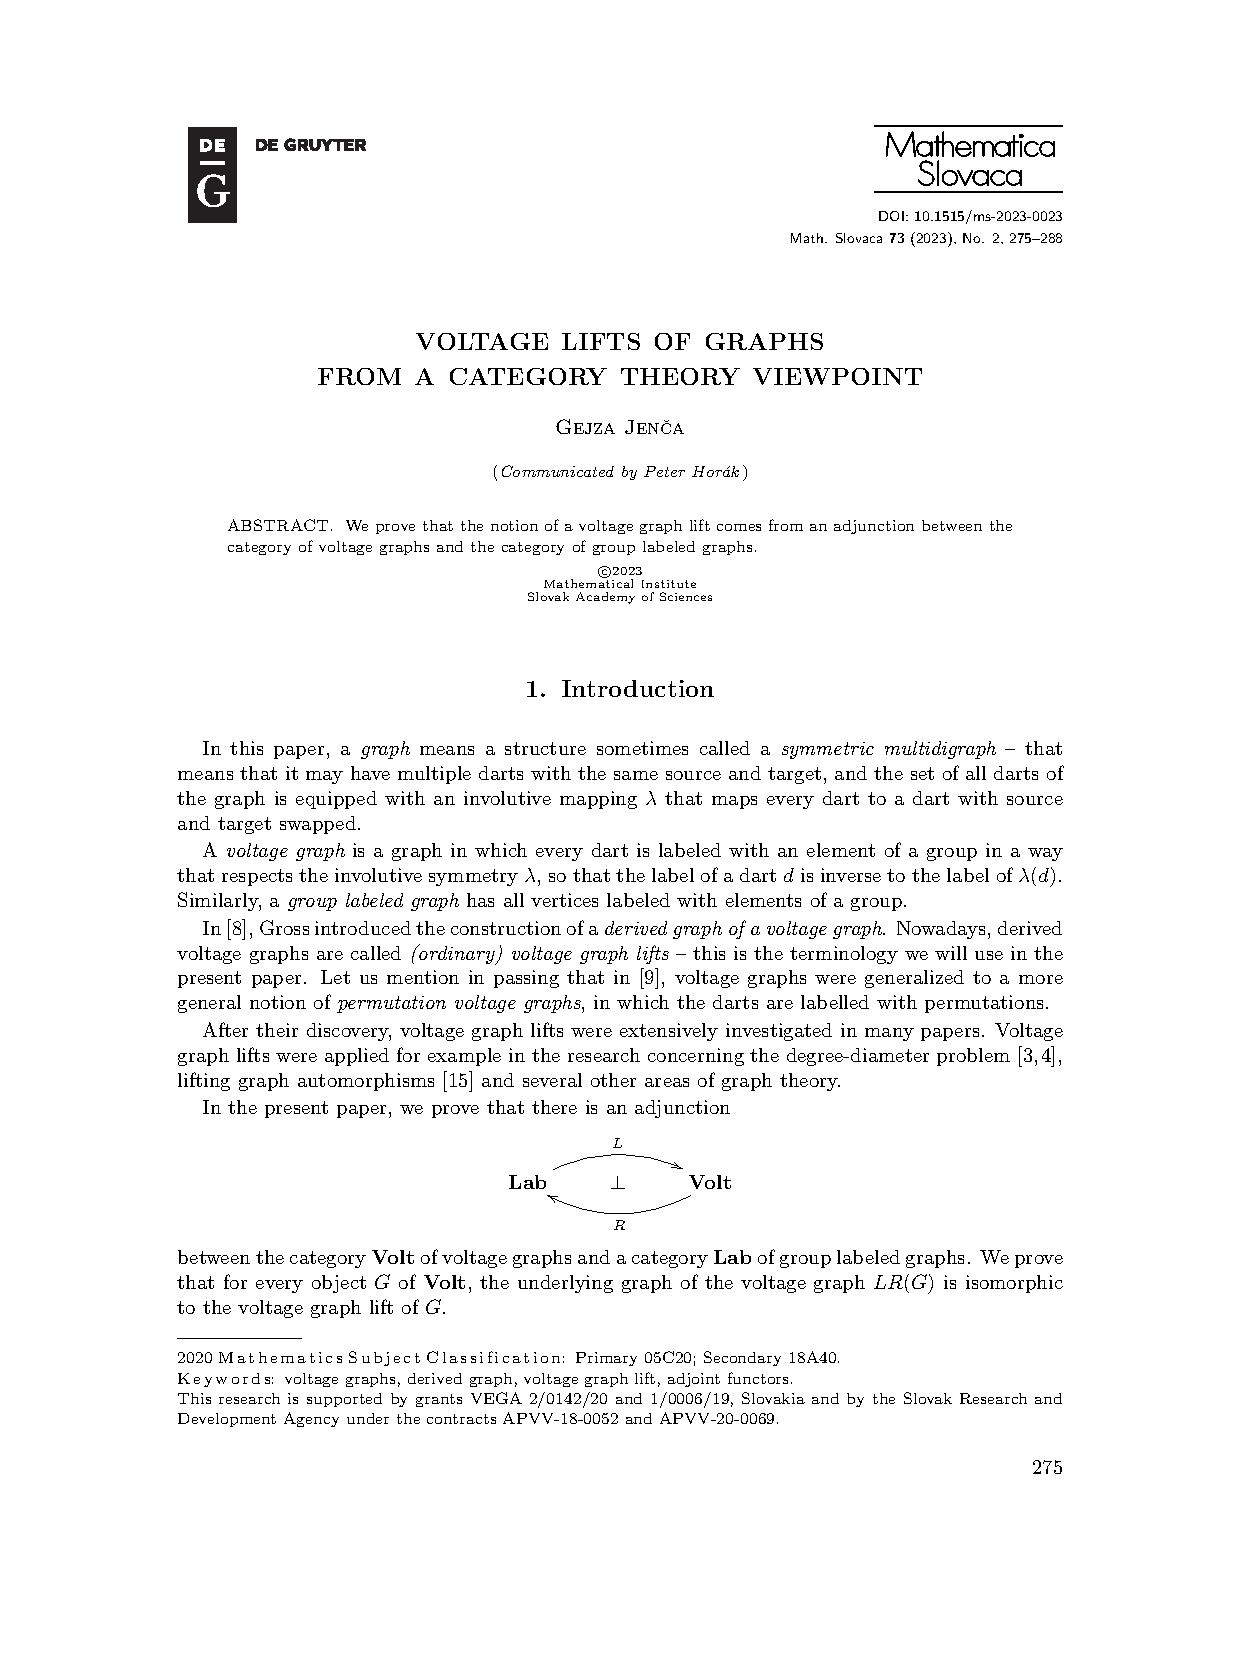
\includegraphics[scale=0.3]{page}
\end{center}
\end{frame}
\begin{frame}
\frametitle{Categories}
\begin{definition}
A \emph{category} $\C$ is a
\begin{itemize}
\item collection of objects $\C_0$, collection of morphisms $\C_1$
\item each morphism $f$ has a domain object and a codomain object 
\[
f\colon A\to B\qquad\xymatrix{A\ar[r]^f &B}
\]
\item for every object $A$ there is an identity morphism $\id_A\colon A\to A$
\item We may compose morphisms
\[
\xymatrix{
A
    \ar[r]^f
    \ar[rd]_{g\circ f}
&
B
    \ar[d]^g
\\
~
&
C
}
\]
\end{itemize}
\end{definition}
\end{frame}
\begin{frame}
\frametitle{Categories}
\framesubtitle{Eilenberg, Mac Lane 1945}
\begin{definition}
\begin{itemize}
\item the composition is associative
\item the $\id_A$ is neutral with respect to composition
\end{itemize}
\end{definition}
Examples: 
\begin{itemize}
\item $\Set,\Grp,\Top,...$
\item Every monoid is a category with a single object.
\item Every poset is a category (at most one morphism between objects)
\end{itemize}
\end{frame}
\begin{frame}
\frametitle{Homsets}
\begin{itemize}
\item For a category $\C$, we write $\C(A,B)$ for the set of all morphisms
with domain $A$ and codomain $B$:
\[
\C(A,B)=\{f\colon A\to B\}
\]
\item Composition is then a mapping
\[
\circ\colon \C(A,B)\times\C(B,C)\to\C(A,C)
\]
\end{itemize}
\end{frame}
\begin{frame}
\frametitle{Functors}
\framesubtitle{morphisms between categories}
A \emph{functor} $F\colon \C\to\D$ is
\begin{itemize}
\item $F(A)\in\D_0$ for each $A\in\C_0$
\item $F(f)\colon F(A)\to F(B)$ for each $(f\colon A\to B)\in\C_1$
\item preserving the composition and the identity morphisms
\[
F(f\circ g)=F(f)\circ F(g)\qquad F(\id_A)=\id_{F(A)}
\]
\end{itemize}
\end{frame}
\begin{frame}
\frametitle{Natural transformations}
\framesubtitle{morphisms between functors}
Let $F,G\colon \C\to\D$ be functors.
A natural transformation $\alpha\colon F\to G$ is
\begin{itemize}
\item For every object $X\in\C_0$
\item a morphism $\alpha_X\colon F(X)\to G(X)$, $\alpha_X\in\D_1$
\item such that for every $f\colon A\to B$ in $\C_1$,
\[
G(f)\circ\alpha_A=\alpha_B\circ F(f)
\]
\[
\xymatrix{
A\ar[r]^f&B
}
\qquad
\xymatrix{
F(A)
    \ar[r]^{F(f)}
    \ar[d]_{\alpha_A}
&
F(B)
    \ar[d]^{\alpha_B}
\\
G(A)
    \ar[r]_{G(f)}
&
G(B)
}
\]
\end{itemize}
\end{frame}
\begin{frame}
\frametitle{Graphs}
A {\em graph} is a quadruple $G=(V,D,s,t,λ)$, where
\begin{itemize}
\item $D$ is the {\em set of darts of $G$}
\item $V$ is the {\em set of vertices of $G$}
\item $s,t\colon D\to V$ are the {\em source and target maps}, respectively.
\item $λ\colon D\to D$ is a mapping such that $λ\circλ=\id_D$.
\item $s\circλ=t$.
\end{itemize}
The mapping $λ$ is called the {\em dart-reversing involution} of $G$.
\end{frame}
\begin{frame}
\frametitle{Graphs}
All the data in a graph $(V,D,s,t,λ)$ can be expressed graphically by a commutative diagram:
\begin{equation}
\xymatrix{
D
	\ar@/^/[rr]^{\id_D}
	\ar[rd]^{λ}
	\ar@/_/[rdd]_{s}
&
~
&
D
	\ar@/^/[ldd]^{s}
\\
~
&
D
	\ar[d]^-{t}
	\ar[ru]^{λ}
\\
~
&
V
\ar@(dl,dr)_{\id_V}
}
\label{diag:G}
\end{equation}

\end{frame}
\begin{frame}
\frametitle{Morphisms of graphs}
A {\em morphism of graphs} $f\colon G\to H$ is a pair of mappings $(f^V,f^D)$, where 
\begin{itemize}
\item $f^V\colon V(G)\to V(H)$
\item $f^D\colon D(G)\to D(H)$
\item for every dart $d\in D(G)$
\begin{align*}
s(f^D(d))&=f^V(s(d))\\
t(f^D(d))&=f^V(t(d))\\
λ(f^D(d))&=f^D(λ(d))
\end{align*}
\end{itemize}

Clearly, graphs equipped with morphisms form a category, denoted by $\Graph$. 
\end{frame}
\begin{frame}
\frametitle{Graphs are functors to $\Set$}
This
\[
\xymatrix{
D
	\ar@/^/[rr]^{\id_D}
	\ar[rd]^{λ}
	\ar@/_/[rdd]_{s}
&
~
&
D
	\ar@/^/[ldd]^{s}
\\
~
&
D
	\ar[d]^-{t}
	\ar[ru]^{λ}
\\
~
&
V
\ar@(dl,dr)_{\id_V}
}
\]
is a category $\gph$ with $\gph_0=\{D,V\}$ and
$\gph_{1}=\{s,t,\lambda,\id_D,\id_V\}$.

A graph $G$ is functor from $\gph$ to $\Set$:
\begin{itemize}
\item $G(D)$ is the set of darts.
\item $G(V)$ is the set of vertices.
\item $G(s),G(t),G(\lambda),...$ are then maps between those sets.
\item The equations are valid, they are valid in $\gph$ and composition
is preserved by the functor $G$.
\end{itemize}
\end{frame}
\begin{frame}
\frametitle{Morphisms of graphs are natural transformations of functors}
That means, for $G,H\colon\gph\to\Set$
\begin{itemize}
\item $f^D\colon G(D)\to H(D)$
\item $f^V\colon G(V)\to H(V)$
\item Naturality square for $s$ (there are similar for $t,\lambda$)
\[
\xymatrix{
D\ar[r]^s&V
}
\qquad
\xymatrix{
G(D)
    \ar[r]^{G(s)}
    \ar[d]_{f^D}
&
G(V)
    \ar[d]^{f^V}
\\
H(D)
    \ar[r]_{H(s)}
&
H(V)
}
\]
\end{itemize}
\end{frame}
\begin{frame}
\frametitle{$\Graph$ is a topos}
As a consequence of this, $\Graph=\Set^\gph$ is a very nice category:
\begin{itemize}
\item $\Graph$ all small limits and colimits.
\item $\Graph$ is exponentially closed.
\item $\Graph$ has a subobject classifier.
\end{itemize}
\end{frame}
\begin{frame}
\frametitle{Voltage graphs}

A {\em voltage graph} over a group $\Gamma$ is a triple $(G,Γ,α)$,
where 
\begin{itemize}
\item $G$ is a graph
\item $Γ$ is a group
\item $α\colon D(G)\to Γ$ is a mapping such that 
$$α(λ(d))=(α(d))^{-1}$$
\end{itemize}
The mapping $α$ is called a {\em $Γ$-voltage on $G$}.
\end{frame}
\begin{frame}
\frametitle{Morphisms of voltage graphs}
\framesubtitle{$Γ$ is fixed}
A morphism of voltage graphs over $\Gamma$ 
\[
f\colon(G,α)\to(G',α')
\]
is a morphism of graphs
$f\colon G\to G'$ that preserves the voltage 
\begin{itemize}
\item for all $d\in D(G)$, $α(d)=α'(f^D(d))$.
\[
\xymatrix{
D(G)
	\ar[rr]^{f^D}
	\ar[rd]_\alpha
&
~
&
D(G')
	\ar[ld]^{\alpha'}
\\
~
&
\Gamma
}
\]
\item The category of voltage graphs over $\Gamma$ is denoted by $\Volt_Γ$.
\end{itemize}
\end{frame}

\begin{frame}
\frametitle{Voltage lift}
\begin{definition}\cite{gross1974voltage}
\label{def:derived} 
Let $(G,Γ,α)$ be a voltage graph. There is a {\em lift of $G$},
denoted by $(G^α,Γ,α')$
\begin{itemize}
\item $V(G^α)=V(G)×Γ$
\item $D(G^α)=D(G)×Γ$
\item $s(d,x)=(s(d),x)$
\item $t(d,x)=(t(d),x.α(d))$
\item $λ(d,x)=(λ(d),x.α(d))$
\item $α(d,x)=α(d)$
\end{itemize}
\end{definition}
\end{frame}
\begin{frame}
\frametitle{An example; the group is $\mathbb Z_3$}
\begin{center}
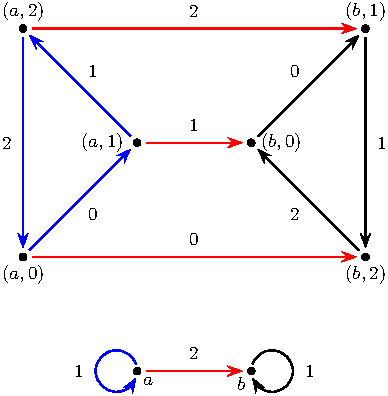
\includegraphics[scale=0.8]{derived1}
\end{center}
\begin{itemize}
\item There is always a projection map: $((a,x)\mapsto a)\colon G^α\to G$
\item The projection map is a very nice surjection (a {\em covering}).
\end{itemize}
\end{frame}
\begin{frame}
\frametitle{Cayley graphs are lifts}
\begin{itemize}
\item Let $S\subseteq\Gamma$ be closed with respect to inversion.
\item $C_S$ is a one-vertex graph with $D(C_S)=S$, $\lambda$ is the inversion.
\item The lift of $C_S$ is the Cayley graph of $S$.
\end{itemize}
\end{frame}
\begin{frame}
\frametitle{Group labeled graphs}
\framesubtitle{We should call them \emph{charge graphs}}
A {\em group labeled graph} 
is a triple $(G,Γ,β)$,
where $G$ is a graph, $Γ$ is a group and $β\colon V(G)\to Γ$ is a mapping, called a {\em $Γ$-labeling on
$G$}.

\end{frame}
\begin{frame}
\frametitle{Morphisms of group labeled graphs}
\framesubtitle{$Γ$ is fixed}
A morphism of $\Gamma$-labeled graphs $(G,β)\to (G',β')$ is a
morphism of graphs $f\colon G\to G'$ such that
for all $v\in V(G)$, $β(v)=β'(f^V(v))$.
\[
\xymatrix{
V(G)
	\ar[rr]^{f^V}
	\ar[rd]_\beta
&
~
&
V(G')
	\ar[ld]^{\beta'}
\\
~
&
\Gamma
}
\]
The category of group labeled graphs is denoted by $\Lab_\Gamma$.
\end{frame}
\begin{frame}
\frametitle{From group labeled graphs to voltage graphs}

For every $\Gamma$-labeled graph $(G,β)$, there is a voltage graph
$L(G,β)=(G,α)$, with the voltage $α$ given by the rule
$α(d)=β(s(d))^{-1}β(t(d))$.
\begin{center}
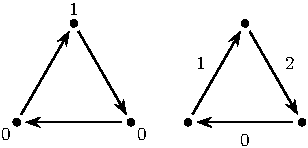
\includegraphics{lleft}
\end{center}
$L$ is a functor $\Lab_\Gamma\to\Volt_\Gamma$.
\end{frame}
\begin{frame}
\frametitle{Can we recognize the objects in the range of $L$?}

\begin{itemize}
\item Which voltage graphs can be represented as $L(G,\beta)$?
\item Not all of them.
\item Obviously, the product of voltages along every closed walk must be 
equal to $1\in\Gamma$.
\item Every voltage lift arises as $L(R(G,\alpha))$ for a certain labelled
graph $R(G,\alpha)$.
\end{itemize}
\end{frame}
\begin{frame}
\frametitle{Adjunction}
\framesubtitle{Kan 1956}
\begin{definition}\cite[(ii) of Theorem IV.1]{mac1998categories}
Let $\C,\D$ be categories and let $F\colon\C\to\D$ and
$G\colon\D\to\C$ be functors. We say that {\em $F$ is left adjoint to $G$},
or that {\em $G$ is right adjoint to $F$}, in symbols $F\isleftadjoint G$, 
if there is a family 
$$
\{\epsilon_Y\colon FG(Y)\to Y\}_{Y\in\obj(\D)}
$$ of $\D$-morphisms,
such that for every $\C$-object $X$ and a $\D$-morphism $f\colon F(X)\to Y$
there is a unique $\C$-morphism $u\colon X\to G(Y)$ such that 
\begin{equation*}
\xymatrix{
F(X)
	\ar[rd]^{f}
	\ar@{.>}[d]_{F(u)}
\\
FG(Y)
	\ar[r]_-{\epsilon_Y}
&
Y
}
\end{equation*}
commutes.
\end{definition}
\end{frame}
\begin{frame}
\frametitle{Adjunction}
For each voltage graph $(G,\alpha)$ over $\Gamma$, we need to find
\begin{itemize}
\item a $\Gamma$-labeled graph $R(G,\alpha)$ and
\item a morphism of voltage graphs $\epsilon_{G,\alpha}\colon L(R(G,\alpha))\to
(G,\alpha)$
\end{itemize}
such that
\begin{itemize}
\item {\color{red}For~every} $\Gamma$-labeled graph $(H,\beta)$ and
\item every morphism of voltage graphs over $\Gamma$ $f:L(H,\beta)\to (G,\alpha)$
\item {\color{red} there~exists~a~unique} morphism of $\Gamma$-labeled graphs 
$u\colon(H,\beta)\to R(G,\alpha)$
\end{itemize}
such that
\[
    \epsilon_{G,\alpha}\circ L(u)=f
\]
\end{frame}

\begin{frame}
\frametitle{Adjunction}
From this, we obtain (for free!)
\begin{itemize}
\item $R$ is a functor
\item $\epsilon\colon (L\circ R)\to \id_{\Volt}$ is a natural transformation:
\[
\xymatrix{
LR(G,\alpha)
    \ar[r]^{LR(f)}
    \ar[d]_{\epsilon_{G,\alpha}}
&
LR(G',\alpha')
    \ar[d]^{\epsilon_{G',\alpha'}}
\\
(G,\alpha)
    \ar[r]_f
&
(G',\alpha')
}
\]
\item $\Volt_\Gamma(L(H),G)\simeq\Lab_\Gamma(H,R(G))$.
\end{itemize}
\end{frame}
\begin{frame}
\frametitle{Adjunctions are \underline{everywhere}}
\[
\adjunction{\Lab_\Gamma}{\Volt_\Gamma}{L}{R}
\]
\[
\adjunction{\Set}{\Rel}{J}{\mathcal{P}}
\]
\[
\adjunction{\Set}{\Grp}{F}{U}
\]
\[
\adjunction{\Set}{\CHaus}{Ult}{U}
\]
\end{frame}
\begin{frame}
\frametitle{A voltage graph is a morphism in $\Graph$}
\begin{itemize}
\item Consider the digraph $\lG$ with a single
vertex $v$ and $D(\lG)=Γ$. 
\item $λ\colon D(\ell(Γ))\to D(\ell(Γ))$ is given by $λ(a)=a^{-1}$. 
\item $\ell$ is then a functor from $\Grp$ to $\Graph$. 
\item A voltage graph $(G,\alpha)$ can be represented as a morphism of graphs
\[
\alpha\colon G\to\ell(\Gamma)
\]
\item Under this representation, morphisms in $\Volt_\Gamma$ are exactly commuting
triangles.
\[
\xymatrix{
G
    \ar[rr]^f
    \ar[rd]_\alpha
&
&
G'
    \ar[ld]^{\alpha'}
\\
&
\ell(\Gamma)
}
\]
\end{itemize}
\end{frame}
\begin{frame}
\frametitle{A group labeled graph is a morphism in $\Graph$}

Let $\Gamma$ be a group. Let $\k(\Gamma)$ be the graph on the vertex set $\Gamma$ with
\begin{itemize}
\item $V(\k(\Gamma))=\Gamma$
\item $D(\k(\Gamma))=\Gamma×\Gamma$
\item $s(x_1,x_2)=x_1$
\item $t(x_1,x_2)=x_2$
\item $λ(x_1,x_2)=(x_2,x_1)$
\end{itemize}
Clearly, $\k$ is a functor from $\Grp$ to $\Graph$. 

A $Γ$-labeling $β$ on
a graph $G$ is the same thing as a morphism of graphs $\beta\colon G\to\KG$.
\end{frame}
\begin{frame}
\frametitle{$L$ as a composition}
For every group, there is a morphism of graphs $q_\Gamma^V\colon\k(\Gamma)\to\ell(\Gamma)$:
\begin{itemize}
\item Every vertex is mapped to the single vertex of $\ell(\Gamma)$.
\item The dart $(a,b)$ in $\k(\Gamma)$ is mapped to the dart $a^{-1}b$ in
$\ell(\Gamma)$.
\item Then, $L$ can be represented as a composition with $q_\Gamma$:
\[
L(G,\beta)=q_\Gamma\circ\beta\qquad
\xymatrix{
G
    \ar[d]_{\beta}
    \ar[rd]^{L(G,\beta)}
\\
\k(\Gamma)
    \ar[r]_{q_\Gamma}
&
\ell(\Gamma)
}
\]
\end{itemize}
\end{frame}
\begin{frame}
\frametitle{R as a pullback along $q_\Gamma$}
\[
\xymatrix{
H
	\ar@/^1.4pc/[rrd]^{f}
	\ar@/_1.4pc/[rdd]_{\beta}
	\ar@{.>}[rd]^{u}
\\
&
R(G)
	\ar[r]^-{\epsilon_{G,\alpha}}
	\ar[d]_{R(\alpha)}
&
G
	\ar[d]^{α}
\\
&
\KG
	\ar[r]_-{q_Γ}
&
\lG
}
\]
\end{frame}
\begin{frame}
\frametitle{The projection is a covering}
An {\em in-neighbourhood} $N(v)$ of a vertex $v$ of a graph is the set
of darts with target $v$.
A morphism of graphs $f\colon G'\to G$ is a {\em fibration}
if for every vertex $v\in V(G')$,
$f^D$ restricted to $N(v)$
is a bijection from $N(v)$ to $N(f(v))$.
A fibration is a {\em covering} if and only if it is surjective on vertices.
\begin{theorem}\cite{boldi2002fibrations}
A morphism of graphs is a fibration iff the square
\[
\xymatrix{
D(G)
	\ar[r]^t
	\ar[d]_{f^D}
&
V(G)
	\ar[d]^{f^V}
\\
D(G')
	\ar[r]_t
&
V(G')
}
\]
is a pullback in $\Set$. A \emph{covering} is a vertex-surjective fibration.
\end{theorem}
\end{frame}
\begin{frame}
\frametitle{The projection is a covering}
\begin{theorem}\cite[Theorem 45]{boldi2002fibrations}
\label{thm:fibrationpullback}
A pullback of a fibration in $\Graph$ along an arbitrary morphism is a fibration.
\end{theorem}
\begin{corollary}
The underlying graph morphism of the projection $\epsilon_{G,\alpha}\colon
R(G,\alpha)\to (G,\alpha)$ is a covering.
\end{corollary}
\begin{proof}
\begin{itemize}
\item $q_\Gamma$ is a fibration.
\item $\epsilon_{G,\alpha}$ is a pullback of $q_{\Gamma}$, and it is surjective.
\end{itemize}
\end{proof}
\end{frame}
\begin{frame}
\hfill
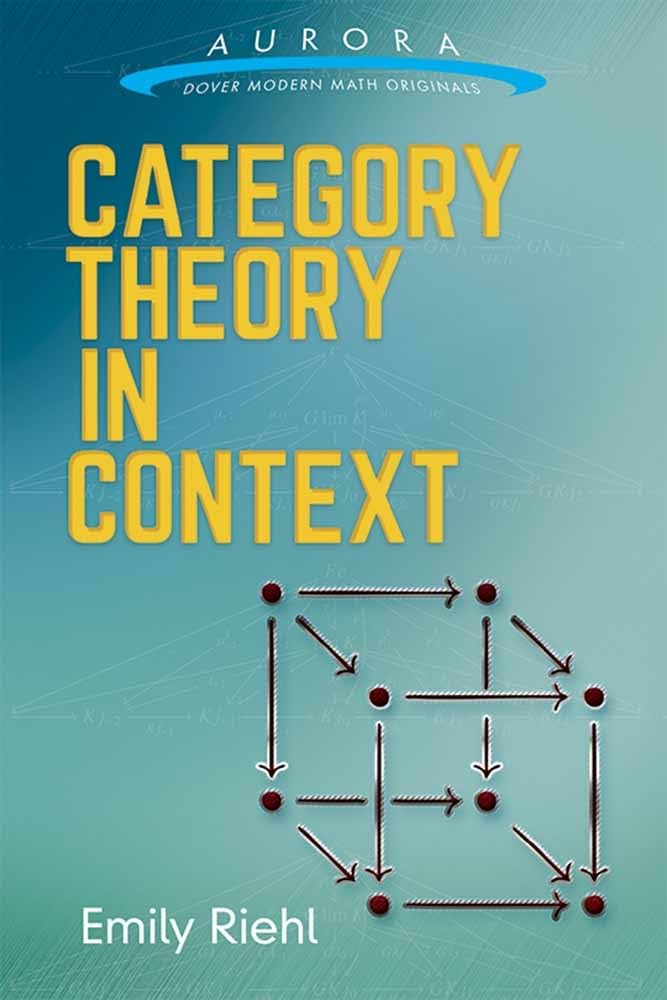
\includegraphics[scale=0.2]{riehl.jpg}
\hfill

\includegraphics[scale=0.4]{leinster.jpg}
\hfill~
\end{frame}
\begin{frame}
\bibliography{mybib}
\bibliographystyle{apalike}
\end{frame}
\end{document}
